\documentclass{article}
\usepackage{graphicx} % Required for inserting images
\usepackage{subfiles}
\usepackage{amsmath,amssymb,amsfonts, amsthm}
\usepackage{bbm}
\usepackage{tikz}
\usepackage{tikz-cd}
\usepackage{mathtools}
\usepackage{xspace}
\usepackage{adjustbox}
\usepackage{todonotes}
\usepackage{mathpartir}
\usepackage{bussproofs}
\usepackage{caption}
\usepackage{svg}
\usepackage{floatrow}

\usepackage{subcaption}
\usepackage{lmodern}
\usepackage{natbib}
\usepackage{xr}
\usepackage{xr-hyper} 
\usepackage[hidelinks]{hyperref}
\usepackage[nameinlink]{cleveref}
\usepackage[symbol]{footmisc}
\usepackage{pdfpages} % Package to include PDF pages
\usepackage{float}

\usepackage[english]{babel}
\usepackage[autostyle, english = american]{csquotes}
\usepackage[lite]{mtpro2}



\DeclareMathAlphabet{\mathbbold}{U}{bbold}{m}{n}
\definecolor{cof}{RGB}{219,144,71}

\newcommand{\id}[1]{\text{id}_{#1}}
\newcommand{\idhom}[1]{\normalfont \text{idhom}_{#1}}
\newcommand{\refl}[1]{\text{refl}_{#1}}
\newcommand{\Un}{\text{Unit}}
\newcommand{\U}{\mathcal{U}}
\newcommand{\vo}{\text{Void}}
\newcommand{\uc}{\U_\text{cov}}
\newcommand{\isc}{\normalfont \text{is\_covariant}}
\newcommand{\dua}{\normalfont \text{dua}}
\newcommand{\dcoe}{\text{dcoe}}
\newcommand{\ho}[3][2]{\normalfont  \text{hom}_{#1}(#2,#3)}
\newcommand{\dho}[4]{\normalfont  \hom_{#1(#2)}(#3, #4)}
\newcommand{\dhot}[5]{\normalfont  \hom^2_{#1(#2)}(#3, #4; #5)}
\newcommand{\hot}[4][]{\ensuremath{\text{hom}^2_{#1}({#2},{#3};{#4})}}
\newcommand{\seg}{\text{seg}}
\newcommand{\defeq}{\vcentcolon\equiv}
\newcommand{\comp}[2]{\text{comp}_{#1, #2}}
\newcommand{\co}{\text{code}}
\newcommand{\eco}{\text{encode}}
\newcommand{\fst}{\text{fst}}
\newcommand{\snd}{\text{snd}}
\newcommand{\dco}{\text{decode}}
\newcommand{\htf}{\normalfont \text{homtofun}}
\newcommand{\funext}{\normalfont \text{funext}}
\newcommand{\happly}{\normalfont \text{happly}}
\newcommand{\cu}{\normalfont \text{cube}}
\newcommand{\tope}{\normalfont \text{tope}}
\newcommand{\dom}{\normalfont \text{dom}}
\newcommand{\cod}{\normalfont \text{cod}}
\newcommand{\two}{\mathbb{2}}
\newcommand{\yon}[2]{\normalfont \text{yon}^{#1}_{#2}}
\newcommand{\trans}[2]{\normalfont \text{trans}_{{#1}, {#2}}}
\newcommand{\qinv}{\normalfont \text{qinv}}
\newcommand{\linv}{\normalfont \text{linv}}
\newcommand{\rinv}{\normalfont \text{rinv}}
\newcommand{\biinv}{\normalfont \text{biinv}}
\newcommand{\iseq}{\normalfont \text{isequiv}}
\newcommand{\tot}{\normalfont \text{total}}

%from RS17
\newcommand{\sh}[2]{\{#1\mid #2\}}
\newcommand{\exten}[4]{\left\langle\mathchoice{\textstyle\prod_{#1}}{\textstyle\prod_{#1}}{\scriptstyle\prod_{#1}}{\scriptscriptstyle\prod_{#1}} #2 \middle|^{#3}_{#4}\right\rangle}
\newcommand{\ndexten}[4]{\left\langle #1 \to #2 \middle|^{#3}_{#4}\right\rangle}

%extension type stuff
\def\pair#1#2{\left \langle #1, #2 \right \rangle}

%simplex stuff
\def\tzhorn{\Lambda_0^2}
\def\tohorn{\Lambda_1^2}
\def\tthorn{\Lambda_2^2}
\def\pardo{\partial\Delta^1}
\def\pardt{\partial\Delta^2}
\def\osx{\Delta^1}

\def\tsx{\Delta^2}

\def\homtwoshort#1(#2,#3,#4,#5,#6,#7){\hom_{#1}^2(#5,#6;#7)}
\def\homtwo#1{\hom_{#1}^2\homtwoarg1}
\def\homtwolong#1#2{\hom_{#2}^2\homtwoarg#1}
\def\homtwoarg#1(#2,#3,#4,#5,#6,#7){\left(
    \begin{tikzpicture}[baseline,xscale=#1]
      \node (a) at (0,0) {$\scriptstyle #2$};
      \node (b) at (1,.3) {$\scriptstyle #3$};
      \node (c) at (2,0) {$\scriptstyle #4$};
      \draw (a) -- node [auto] {$\scriptstyle #5$} (b);
      \draw (b) -- node [auto] {$\scriptstyle #6$} (c);
      \draw (a) -- node [auto,swap] {$\scriptstyle #7$} (c);
    \end{tikzpicture}\right)}


%https://tex.stackexchange.com/questions/325297/how-to-scale-a-tikzcd-diagram


%%book hott%%

%%% Dependent products %%%
\def\prdsym{\textstyle\prod}
%% Call the macro like \prd{x,y:A}{p:x=y} with any number of
%% arguments.  Make sure that whatever comes *after* the call doesn't
%% begin with an open-brace, or it will be parsed as another argument.
\makeatletter
% Currently the macro is configured to produce
%     {\textstyle\prod}(x:A) \; {\textstyle\prod}(y:B),{\ }
% in display-math mode, and
%     \prod_{(x:A)} \prod_{y:B}
% in text-math mode.
% \def\prd#1{\@ifnextchar\bgroup{\prd@parens{#1}}{%
%     \@ifnextchar\sm{\prd@parens{#1}\@eatsm}{%
%         \prd@noparens{#1}}}}
\def\prd#1{\@ifnextchar\bgroup{\prd@parens{#1}}{%
    \@ifnextchar\sm{\prd@parens{#1}\@eatsm}{%
    \@ifnextchar\prd{\prd@parens{#1}\@eatprd}{%
    \@ifnextchar\;{\prd@parens{#1}\@eatsemicolonspace}{%
    \@ifnextchar\\{\prd@parens{#1}\@eatlinebreak}{%
    \@ifnextchar\narrowbreak{\prd@parens{#1}\@eatnarrowbreak}{%
      \prd@noparens{#1}}}}}}}}
\def\prd@parens#1{\@ifnextchar\bgroup%
  {\mathchoice{\@dprd{#1}}{\@tprd{#1}}{\@tprd{#1}}{\@tprd{#1}}\prd@parens}%
  {\@ifnextchar\sm%
    {\mathchoice{\@dprd{#1}}{\@tprd{#1}}{\@tprd{#1}}{\@tprd{#1}}\@eatsm}%
    {\mathchoice{\@dprd{#1}}{\@tprd{#1}}{\@tprd{#1}}{\@tprd{#1}}}}}
\def\@eatsm\sm{\sm@parens}
\def\prd@noparens#1{\mathchoice{\@dprd@noparens{#1}}{\@tprd{#1}}{\@tprd{#1}}{\@tprd{#1}}}
% Helper macros for three styles
\def\lprd#1{\@ifnextchar\bgroup{\@lprd{#1}\lprd}{\@@lprd{#1}}}
\def\@lprd#1{\mathchoice{{\textstyle\prod}}{\prod}{\prod}{\prod}({\textstyle #1})\;}
\def\@@lprd#1{\mathchoice{{\textstyle\prod}}{\prod}{\prod}{\prod}({\textstyle #1}),\ }
\def\tprd#1{\@tprd{#1}\@ifnextchar\bgroup{\tprd}{}}
\def\@tprd#1{\mathchoice{{\textstyle\prod_{(#1)}}}{\prod_{(#1)}}{\prod_{(#1)}}{\prod_{(#1)}}}
\def\dprd#1{\@dprd{#1}\@ifnextchar\bgroup{\dprd}{}}
\def\@dprd#1{\prod_{(#1)}\,}
\def\@dprd@noparens#1{\prod_{#1}\,}

%%% Dependent sums %%%
\def\smsym{\textstyle\sum}
% Use in the same way as \prd
\def\sm#1{\@ifnextchar\bgroup{\sm@parens{#1}}{%
    \@ifnextchar\prd{\sm@parens{#1}\@eatprd}{%
    \@ifnextchar\sm{\sm@parens{#1}\@eatsm}{%
    \@ifnextchar\;{\sm@parens{#1}\@eatsemicolonspace}{%
    \@ifnextchar\\{\sm@parens{#1}\@eatlinebreak}{%
    \@ifnextchar\narrowbreak{\sm@parens{#1}\@eatnarrowbreak}{%
        \sm@noparens{#1}}}}}}}}
\def\sm@parens#1{\@ifnextchar\bgroup%
  {\mathchoice{\@dsm{#1}}{\@tsm{#1}}{\@tsm{#1}}{\@tsm{#1}}\sm@parens}%
  {\@ifnextchar\prd%
    {\mathchoice{\@dsm{#1}}{\@tsm{#1}}{\@tsm{#1}}{\@tsm{#1}}\@eatprd}%
    {\mathchoice{\@dsm{#1}}{\@tsm{#1}}{\@tsm{#1}}{\@tsm{#1}}}}}
\def\@eatprd\prd{\prd@parens}
\def\sm@noparens#1{\mathchoice{\@dsm@noparens{#1}}{\@tsm{#1}}{\@tsm{#1}}{\@tsm{#1}}}
\def\lsm#1{\@ifnextchar\bgroup{\@lsm{#1}\lsm}{\@@lsm{#1}}}
\def\@lsm#1{\mathchoice{{\textstyle\sum}}{\sum}{\sum}{\sum}({\textstyle #1})\;}
\def\@@lsm#1{\mathchoice{{\textstyle\sum}}{\sum}{\sum}{\sum}({\textstyle #1}),\ }
\def\tsm#1{\@tsm{#1}\@ifnextchar\bgroup{\tsm}{}}
\def\@tsm#1{\mathchoice{{\textstyle\sum_{(#1)}}}{\sum_{(#1)}}{\sum_{(#1)}}{\sum_{(#1)}}}
\def\dsm#1{\@dsm{#1}\@ifnextchar\bgroup{\dsm}{}}
\def\@dsm#1{\sum_{(#1)}\,}
\def\@dsm@noparens#1{\sum_{#1}\,}


%%% Map on paths %%%
\newcommand{\mapfunc}[1]{\ensuremath{\mathsf{map}_{#1}}\xspace} % Without argument
\newcommand{\map}[2]{\ensuremath{{#1}\mathopen{}\left({#2}\right)\mathclose{}}\xspace}
\let\Ap\map
%\newcommand{\Ap}[2]{\ensuremath{{#1}\left({#2}\right)}\xspace}
\newcommand{\mapdepfunc}[1]{\ensuremath{\mathsf{apd}_{#1}}\xspace} % Without argument
% \newcommand{\mapdep}[2]{\ensuremath{{#1}\llparenthesis{#2}\rrparenthesis}\xspace}
\newcommand{\mapdep}[2]{\ensuremath{\mapdepfunc{#1}\mathopen{}\left(#2\right)\mathclose{}}\xspace}

%%% 2D map on paths
\newcommand{\aptwofunc}[1]{\ensuremath{\mathsf{ap}^2_{#1}}\xspace}
\newcommand{\aptwo}[2]{\ensuremath{\aptwofunc{#1}\mathopen{}\left({#2}\right)\mathclose{}}\xspace}
\newcommand{\apdtwofunc}[1]{\ensuremath{\mathsf{apd}^2_{#1}}\xspace}
\newcommand{\apdtwo}[2]{\ensuremath{\apdtwofunc{#1}\mathopen{}\left(#2\right)\mathclose{}}\xspace}

%%% Lambda abstractions.
% Each variable being abstracted over is a separate argument.  If
% there is more than one such argument, they *must* be enclosed in
% braces.  Arguments can be untyped, as in \lam{x}{y}, or typed with a
% colon, as in \lam{x:A}{y:B}. In the latter case, the colons are
% automatically noticed and (with current implementation) the space
% around the colon is reduced.  You can even give more than one variable
% the same type, as in \lam{x,y:A}.
\def\lam#1{{\lambda}\@lamarg#1:\@endlamarg\@ifnextchar\bgroup{.\,\lam}{.\,}}
\def\@lamarg#1:#2\@endlamarg{\if\relax\detokenize{#2}\relax #1\else\@lamvar{\@lameatcolon#2},#1\@endlamvar\fi}
\def\@lamvar#1,#2\@endlamvar{(#2\,{:}\,#1)}
% \def\@lamvar#1,#2{{#2}^{#1}\@ifnextchar,{.\,{\lambda}\@lamvar{#1}}{\let\@endlamvar\relax}}
\def\@lameatcolon#1:{#1}
\let\lamt\lam
% This version silently eats any typing annotation.
\def\lamu#1{{\lambda}\@lamuarg#1:\@endlamuarg\@ifnextchar\bgroup{.\,\lamu}{.\,}}
\def\@lamuarg#1:#2\@endlamuarg{#1}

% Function definition with domain and codomain
\newcommand{\function}[4]{\left\{\begin{array}{rcl}#1 &
      \longrightarrow & #2 \\ #3 & \longmapsto & #4 \end{array}\right.}



%%%shit i nabbed from book hott
%%% Map on morphisms %%%
\newcommand{\maparrfunc}[1]{\ensuremath{\mathsf{map}^{\rightarrow}_{#1}}\xspace} % Without argument
\newcommand{\maparr}[2]{\ensuremath{{#1}\mathopen{}\left({#2}\right)\mathclose{}}\xspace}
\let\ap\maparr

%%% 2D map on paths
\newcommand{\apatwofunc}[1]{\ensuremath{\mathsf{ap}^{2\rightarrow}_{#1}}\xspace}
% \newcommand{\aptwo}[2]{\ensuremath{\aptwofunc{#1}\mathopen{}\left({#2}\right)\mathclose{}}\xspace}
% \newcommand{\apdtwofunc}[1]{\ensuremath{\mathsf{apd}^2_{#1}}\xspace}
% \newcommand{\apdtwo}[2]{\ensuremath{\apdtwofunc{#1}\mathopen{}\left(#2\right)\mathclose{}}\xspace}

%%% Bracket/squash/truncation types %%%
\newcommand{\trunc}[2]{\mathopen{}\left\Vert #2\right\Vert_{#1}\mathclose{}}

%%% Equivalence types %%%
\newcommand{\hfib}[2]{{\mathsf{fib}}_{#1}(#2)}

%%% Map on paths %%%
\newcommand{\apfunc}[1]{\ensuremath{\mathsf{ap}_{#1}}\xspace} % Without argument

%% random

%https://tex.stackexchange.com/questions/273034/square-version-of-cdot-small-black-square
\newcommand*\sq{\mathbin{\vcenter{\hbox{\rule{.3ex}{.3ex}}}}}

\newtheoremstyle{named}{}{}{\itshape}{}{\bfseries}{.}{.5em}{\thmnote{#3's }#1}

\newtheorem{theorem}{Theorem}[subsection]
\newtheorem{proposition}[theorem]{Proposition}
\newtheorem{corollary}{Corollary}[theorem]
\newtheorem{lemma}[theorem]{Lemma}
\newtheorem{axiom}[theorem]{Axiom}
\newlength{\perspective}

\crefname{lemma}{lemma}{lemmas}
\crefname{corollary}{corollary}{corollaries}

\theoremstyle{named}
\newtheorem*{namedaxiom}{Axiom}
\newtheorem{namedlemma}[theorem]{Lemma}

\theoremstyle{remark}
\newtheorem*{remark}{Remark}

\theoremstyle{definition}
\newtheorem{definition}[theorem]{Definition}
\newenvironment{dedication}
    {\vspace{6ex}\begin{quotation}\begin{center}\begin{em}}
    {\par\end{em}\end{center}\end{quotation}}


\providecommand{\lemmaautorefname}{Lemma}

\begin{document}

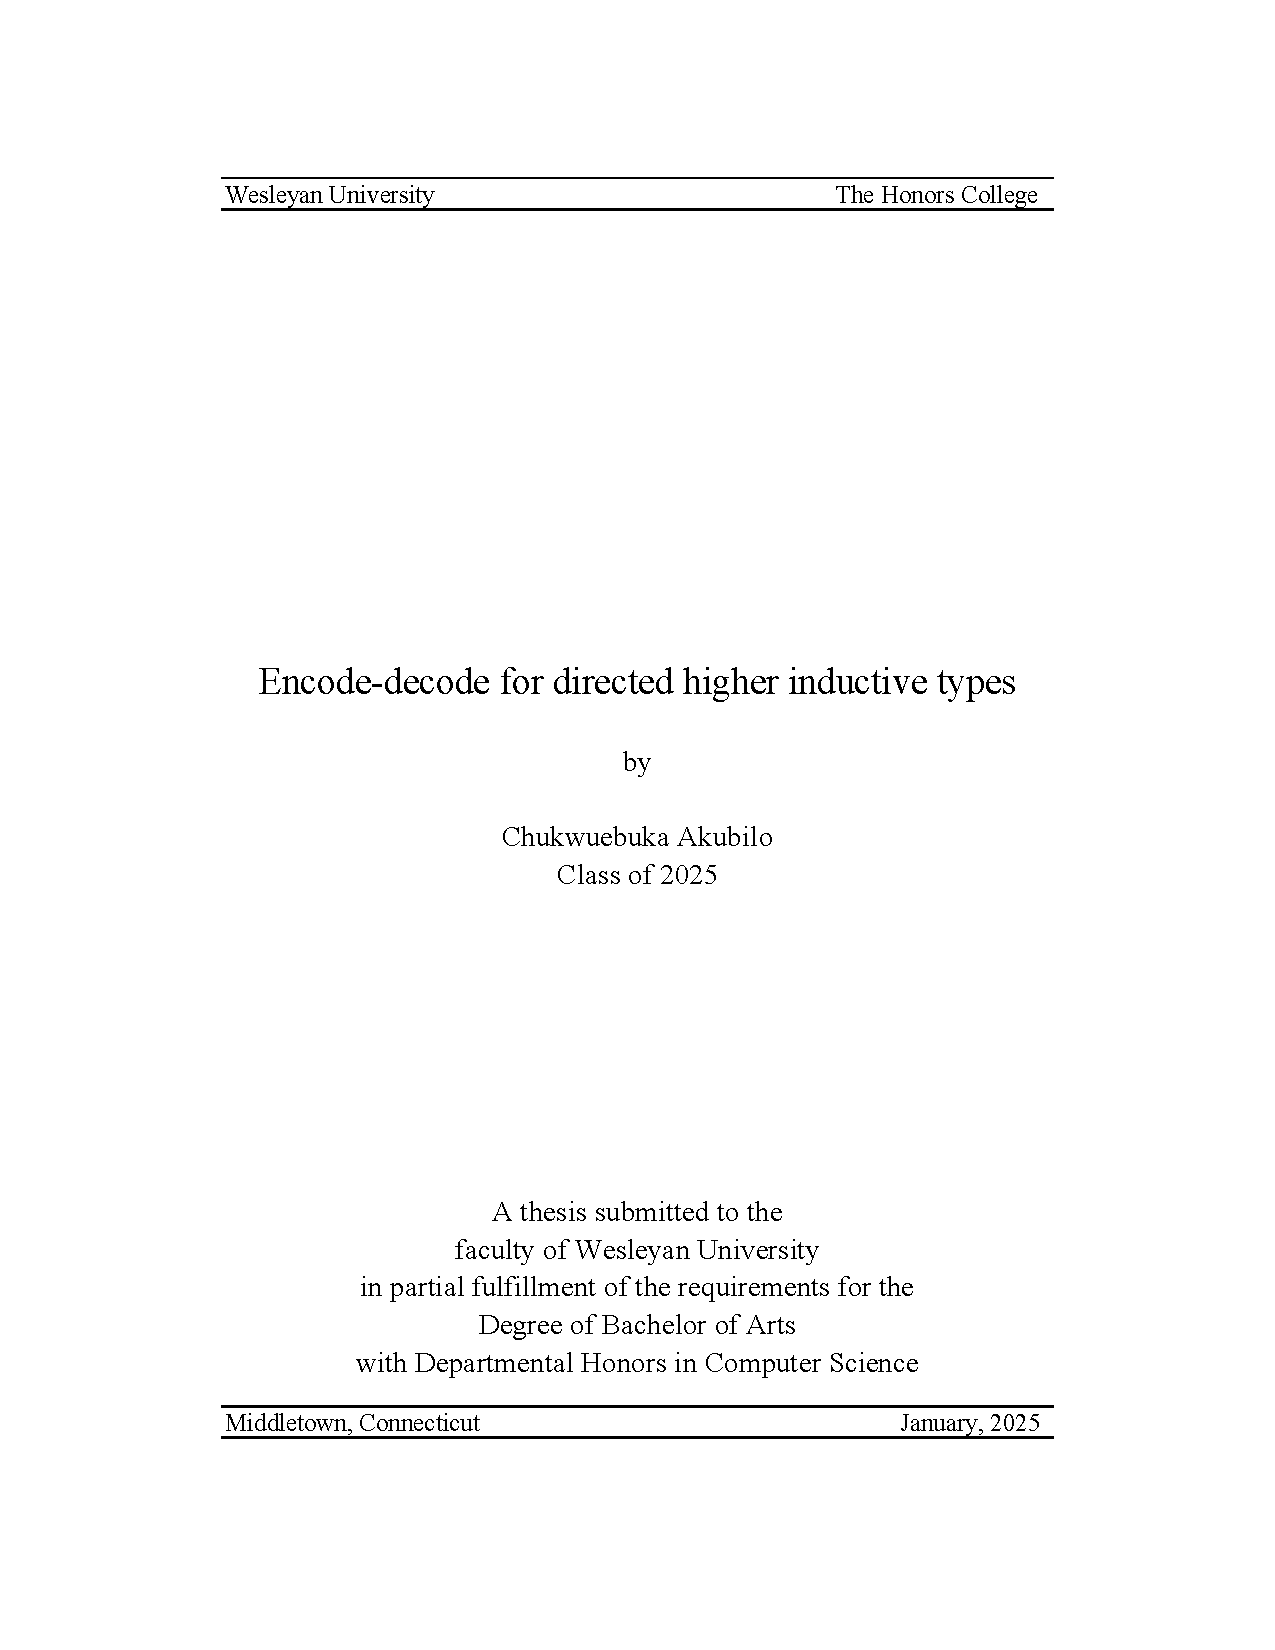
\includepdf[pages=1]{body/thesis-first-page.pdf}

%preamble
\clearpage

\thispagestyle{empty}
\null\vfill
\begin{quote}
    \itshape
    As an empiricist I continue to think of the conceptual scheme of science as a tool, ultimately, for predicting future experience
    in the light of past experience. Physical objects are conceptually imported into the situation as convenient intermediaries—not
    by definition in terms of experience, but simply as irreducible posits comparable, epistemologically, to the gods of Homer. 
    Let me interject that for my part I do, \textit{qua} lay physicist, believe in physical objects and not in Homer’s gods; and I
    consider it a scientific error to believe otherwise. But in point of epistemological footing the physical objects and the 
    gods differ only in degree and not in kind. Both sorts of entities enter our conception only as cultural posits. The myth of
    physical objects is epistemologically superior to most in that it has proved more efficacious than other myths as a device
    for working a manageable structure into the flux of experience.

    \end{quote}
    
    \begin{flushright}
    \textbf{Two Dogmas of Empiricism, W. V. O. Quine}
    \end{flushright}

\vfill\vfill

\clearpage

\subsection*{\centering Acknowledgements}
\addcontentsline{toc}{section}{Acknowledgements}
\subfile{body/0. acknowledgements}
\newpage
\begin{abstract}
Homotopy Type Theory (HoTT) extends Martin-Löf Type Theory (MLTT) with new axioms and type constructors that facilitate the study of \(\infty\)-groupoids and enable a homotopical interpretation of type theory. In this interpretation, the equality type is viewed as a \textit{path} in a topological space, and type families are considered fibrations. Central to this framework is \textit{Voevodsky's univalence axiom}, which formalizes the mathematical shorthand that identifies isomorphic objects as equal. This axiom allows equivalences between types (\(A \simeq B\)) to be lifted along type families to equivalences (\(C(A) \simeq C(B)\)). Additionally, HoTT incorporates \textit{higher inductive types}, which are defined inductively using both point and \textit{path} constructors, enabling the construction of free groupoids such as the interval, the circle, homotopy pushouts, and colimits.

Simplicial Type Theory (STT) builds on HoTT by introducing additional layers for constructing polytopes out of products of the directed interval \(\mathbbm{2}\). This extension allows for the exploration of categorical structures, including morphisms, 2-morphisms, and higher morphisms. This thesis assumes a classifying universe for covariant fibrations (\(\mathcal{U}_c\)) and \textit{directed univalence} to define and prove statements about \textit{directed higher inductive types}. The universe \(\mathcal{U}_c\) enables the treatment of type families with codomain \(\mathcal{U}_c\) as covariant fibrations. Directed univalence generalizes the univalence axiom by formalizing the notion that morphisms between types are functions, thus facilitating the study of concrete categories within type theory. Directed higher inductive types extend the inductive type schema to include \textit{morphism} constructors, supporting the construction of free categories.

This thesis explores the construction of free categories such as the directed interval and the simplicial circle. These extensions highlight the potential of STT to provide a robust framework for studying categorical structures in a homotopical and directed context.
\end{abstract}
\newpage
\tableofcontents

\newpage 
\subsection*{\centering Introduction}
\addcontentsline{toc}{section}{Introduction}
\subfile{body/Introduction}
\newpage
\section*{\centering 1. HoTT}

In this section, we delve into the foundational elements of HoTT, laying the groundwork for our exploration of directed type theory in subsequent sections. We will begin by examining the core concept of paths within types, which are fundamental to the homotopical interpretation of type theory. Building upon this, we will introduce homotopies, which provide a way to relate paths, and equivalences, a key notion for establishing sameness between types. These concepts are essential for understanding how HoTT captures higher-dimensional structures. We then explore how specific classes of types, namely sets and types representing propositions, are characterized within this framework. Finally, we will investigate properties of dependent pair types, also known as $\Sigma$-types, and establish some fundamental lemmas about them that will be useful in later sections. 

\addcontentsline{toc}{section}{1. HoTT}
\setcounter{section}{1}
\stepcounter{subsection}

\subsection*{1.1 Types are higher groupoids}
\addcontentsline{toc}{subsection}{1. Types are higher groupoids}
\subfile{body/1. HoTT/THG}
\stepcounter{subsection}

\subsection*{1.2 Functions are functors}
\addcontentsline{toc}{subsection}{2. Functions are functors}
\subfile{body/1. HoTT/FAF}
\stepcounter{subsection}

\subsection*{1.3 Type families are fibrations}
\addcontentsline{toc}{subsection}{3. Type families are fibrations}
\subfile{body/1. HoTT/TFAF}
\stepcounter{subsection}



\subsection*{1.4 Homotopies and equivalences}
\addcontentsline{toc}{subsection}{4. Homotopies and Equivalences}
\subfile{body/1. HoTT/HomotopiesAndEquivalences}
\stepcounter{subsection}


\subsection*{1.5 Sets and Logic}
\addcontentsline{toc}{subsection}{5. Sets and Logic}
\subfile{body/1. HoTT/SAL}
\stepcounter{subsection}

\subsection*{1.6 Univalence}
\addcontentsline{toc}{subsection}{6. Univalence}
\subfile{body/1. HoTT/univalence}
\stepcounter{subsection}

\subsection*{1.7 $\Pi$-types}
\addcontentsline{toc}{subsection}{7. $\Pi$-types}
\subfile{body/1. HoTT/pitypes}
\stepcounter{subsection}

\subsection*{1.8 $\Sigma$-types}
\addcontentsline{toc}{subsection}{8. $\Sigma$-types}
\subfile{body/1. HoTT/sigmatypes}
\stepcounter{subsection}

\newpage

\section*{\centering 2. sHoTT}
\addcontentsline{toc}{section}{2. sHoTT}
\setcounter{section}{2}
\setcounter{equation}{0}
\setcounter{theorem}{0}
\setcounter{subsection}{1}

Simplicial homotopy type theory extends HoTT with \textit{extension types} and two extra layers, turning it into a
 \textit{type theory with shapes}. It is specialized to the case of a cube $\mathbbm{2}$ and an inequality tope, including rules making the tope layer the coherent logic\footnote{A coherent logic is a fragment of first-order logic that only allows the quantifiers and connectives $\lor$, $\land$, $\top$, $\bot$, and $\exists$.} of a strict interval. The top geometric layers interact with the bottom type theory layer
 through extension types. Extension types allow us to introduce dependent functions whose domain is a shape. To introduce an extension type, a shape that includes into the domain shape, a term that depends on that shape must be provided. Then, the extension
 type can be thought of as extending the provided section from a partial domain to a full domain. 

 With extension types in tow, we can probe simplicial shapes in types. That is, we can probe morphisms, 2-morphisms, 3-morphisms and higher by defining the right extension type. Using familiar notions from HoTT, we can then define a class of types whose morphisms have a weak composition structure, \textit{Segal types}. Segal types are a useful model of the notion of category. We can also define a type of classes that has no interesting simplicial data. These types are ones where the path types and morphism types are equivalent, they are dubbed \textit{discrete types}. Extending this further, types whose \textit{isomorphisms} are equivalent to its paths are dubbed \textit{Rezk types}. 


We can also reflect our situation in HoTT in sHoTT. In HoTT, all type families are fibrations. In sHoTT, \textit{some} type families are fibrations. We can define the type of type families that lift morphisms covariantly and contravariantly, which are aptly dubbed \textit{covariant} and \textit{contravariant type families}. We are not limited to lifting morphisms, we call families that lift 2-morphisms \textit{inner type families}. 

As mentioned before, we are working in a bespoke simplicial homotopy type theory. Included in our extended sHoTT is a Segal classifying universe of covariant fibrations. We also include a directed univalence axiom which allows us to turn morphisms between discrete types into functions between them. 

In this section, we give an informal introduction to sHoTT and develop machinery for use in Section 4.
\subsection*{2.1 Three-layer type theory with shapes}
\addcontentsline{toc}{subsection}{1. Three-layer type theory with shapes}
\subfile{body/2. sHoTT/Three-layer_type_theory_with_shapes}
\setcounter{theorem}{0}
\stepcounter{subsection}


\subsection*{2.2 Extension types}
\addcontentsline{toc}{subsection}{2. Extension types}
\subfile{body/2. sHoTT/Extension_Types}
\setcounter{theorem}{0}
\stepcounter{subsection}


\subsection*{2.3 Segal condition}
\addcontentsline{toc}{subsection}{3. Segal condition}
\subfile{body/2. sHoTT/Segalcondition}
\setcounter{theorem}{0}
\stepcounter{subsection}

\subsection*{2.4 Discrete types}
\addcontentsline{toc}{subsection}{4. Discrete types}
\subfile{body/2. sHoTT/Discretetypes}
\setcounter{theorem}{0}
\stepcounter{subsection}

\subsection*{2.5 Rezk types}
\addcontentsline{toc}{subsection}{5. Rezk types}
\subfile{body/2. sHoTT/rezk}
\setcounter{theorem}{0}
\stepcounter{subsection}

\subsection*{2.6 Covariant fibrations}
\addcontentsline{toc}{subsection}{6. Covariant fibrations}
\subfile{body/2. sHoTT/Covariantfibrations}
\setcounter{theorem}{0}
\stepcounter{subsection}

\subsection*{2.7 Yoneda lemma}
\addcontentsline{toc}{subsection}{7. Yoneda Lemma}
\subfile{body/2. sHoTT/yoneda}
\setcounter{theorem}{0}
\stepcounter{subsection}

\subsection*{2.8 Directed univalence}
\addcontentsline{toc}{subsection}{8. Directed univalence}
\subfile{body/2. sHoTT/Directedunivalence}
\setcounter{theorem}{0}
\stepcounter{subsection}


\subsection*{2.9 Inner fibrations}
\addcontentsline{toc}{subsection}{9. Inner fibrations}
\subfile{body/2. sHoTT/Innerfibrations}
\setcounter{theorem}{0}
\stepcounter{subsection}



\section{Directed Higher Inductive Types}
\setcounter{section}{3}
\setcounter{equation}{0}
\setcounter{theorem}{0}
\setcounter{subsection}{1}
In this section, we start our investigation of directed higher inductive types, starting at types that have no simplicial data
to types that have more complicated structure. For these types, our main object of study is the generalization of the fundamental groupoid 
of a space: the \textbf{fundamental monoid} of a category.
\addcontentsline{toc}{subsection}{1. Inductive Types in sHoTT}
\subsection*{3.1 Inductive types in sHoTT}
\subfile{body/3. Directed Higher Inductive Types/inductivetypes}
\setcounter{theorem}{0}
\stepcounter{subsection}

\addcontentsline{toc}{subsection}{2. Directed Interval}
\subsection*{3.2 Directed Interval}
\subfile{body/3. Directed Higher Inductive Types/directedinterval}
\setcounter{theorem}{0}
\stepcounter{subsection}

\addcontentsline{toc}{subsection}{3. Directed Circle}
\subsection*{3.3 Directed Circle}
\subfile{body/3. Directed Higher Inductive Types/directedcircle}
\setcounter{theorem}{0}
\stepcounter{subsection}
\newpage

\subsection*{\centering Appendix}
\addcontentsline{toc}{section}{Appendix}
\begin{figure}[h]
    \centering
    \begin{mathpar}
      \inferrule{ }{\unittype \cube}\and
      \inferrule{I\cube \\ J\cube}{I\times J\cube}\and
      \inferrule{(t:I)\in \Xi}{\Xi\types t:I}\and
      \inferrule{ }{\Xi\types\star:\unittype}\\
      \inferrule{\Xi\types s:I \\ \Xi\types t:J}{\Xi\types \pair{s,t}:I\times J}\and
      \inferrule{\Xi\types t:I\times J}{\Xi\types \pi_1(t):I}\and
      \inferrule{\Xi\types t:I\times J}{\Xi\types \pi_2(t):J}\and
    \end{mathpar}
    \caption{The cube layer}
    \label{fig:cubes}
  \end{figure}

\begin{figure}
    \centering
    \begin{mathpar}
      \inferrule{\phi\in \Phi}{\Xi\mid\Phi\types \phi}\and
      \inferrule{ }{\Xi\types \top\tope}\and
      \inferrule{ }{\Xi\mid \Phi \types \top}\and
      \inferrule{ }{\Xi\types \bot\tope}\and
      \inferrule{\Xi\mid\Phi\types \bot}{\Xi\mid\Phi\types \psi}\and
      \inferrule{\Xi\types \phi\tope \\ \Xi\types \psi\tope}{\Xi\types (\phi\land\psi)\tope}\and
      \inferrule{\Xi\mid\Phi\types \phi \\ \Xi\mid\Phi\types \psi}{\Xi\mid\Phi\types \phi\land\psi}\and
      \inferrule{\Xi\mid\Phi\types \phi\land\psi}{\Xi\mid\Phi\types \phi}\and
      \inferrule{\Xi\mid\Phi\types \phi\land\psi}{\Xi\mid\Phi\types \psi}\and
      \inferrule{\Xi\types \phi\tope \\ \Xi\types \psi\tope}{\Xi\types (\phi\lor\psi)\tope}\and
      \inferrule{\Xi\mid\Phi\types \phi}{\Xi\mid\Phi\types \phi\lor\psi}\and
      \inferrule{\Xi\mid\Phi\types \psi}{\Xi\mid\Phi\types \phi\lor\psi}\and
      \inferrule{\Xi\mid\Phi,\phi\types \chi \\ \Xi\mid\Phi,\psi\types\chi \\ \Xi\mid\Phi\types \phi\lor\psi}{\Xi\mid\Phi\types\chi}\and
      \inferrule{\Xi\types s:I \\ \Xi\types t:I}{\Xi\types (s\jdeq t)\tope}\and
      \inferrule{\Xi\types s:I}{\Xi\mid\Phi\types (s\jdeq s)}\and
      \inferrule{\Xi\mid\Phi\types (s\jdeq t)}{\Xi\mid\Phi\types (t\jdeq s)}\and
      \inferrule{\Xi\mid\Phi\types (s\jdeq t) \\ \Xi\mid\Phi\types (t\jdeq v)}{\Xi\mid\Phi\types (s\jdeq v)}\and
      \inferrule{\Xi\mid\Phi\types (s\jdeq t) \\ \Xi,x:I \types \psi\tope \\ \Xi\mid\Phi\types \psi[s/x]}{\Xi\mid\Phi\types \psi[t/x]}\and
      \inferrule{\Xi\types t:\unittype}{\Xi\mid\Phi\types t\jdeq\star}\and
      \inferrule{\Xi\types s:I \\ \Xi\types t:J}{\Xi\mid\Phi\types \pi_1(\pair{s,t}) \jdeq s}\and
      \inferrule{\Xi\types s:I \\ \Xi\types t:J}{\Xi\mid\Phi\types \pi_2(\pair{s,t}) \jdeq t}\and
      \inferrule{\Xi\types t:I\times J}{\Xi\mid\Phi\types t \jdeq \pair{\pi_1(t),\pi_2(t)}}\and
    \end{mathpar}
    \caption{The tope layer}
    \label{fig:topes}
  \end{figure}

  \begin{figure}
    \centering
    \begin{mathpar}
      \inferrule{\Xi\mid\Phi\types \bot}{\Xi\mid\Phi\mid\Gamma\types \rec_\bot : A}\and
      \inferrule{\Xi\mid\Phi\types \bot \\ \Xi\mid\Phi\mid\Gamma\types a:A}{\Xi\mid\Phi\mid\Gamma\types a\jdeq \rec_\bot}\and
      \inferrule{
        \Xi\mid\Phi\types \phi\lor\psi \\
        \Xi\mid\Phi\mid\Gamma\types A\type \\
        \Xi\mid\Phi,\phi\mid\Gamma\types a_\phi:A \\
        \Xi\mid\Phi,\psi\mid\Gamma\types a_\psi:A \\
        \Xi\mid\Phi,\phi\land\psi\mid\Gamma\types a_\phi \jdeq a_\psi
      }{\Xi\mid\Phi\mid\Gamma\types \rec_\lor^{\phi,\psi}(a_\phi,a_\psi) : A}\and
      \inferrule{
        \Xi\mid\Phi\types \phi\lor\psi \\
        \Xi\mid\Phi\mid\Gamma\types A\type \\
        \Xi\mid\Phi,\phi\mid\Gamma\types a_\phi:A \\
        \Xi\mid\Phi,\psi\mid\Gamma\types a_\psi:A \\
        \Xi\mid\Phi,\phi\land\psi\mid\Gamma\types a_\phi \jdeq a_\psi
      }{\Xi\mid\Phi,\phi\mid\Gamma\types \rec_\lor^{\phi,\psi}(a_\phi,a_\psi) \jdeq a_\phi}\and
      \inferrule{
        \Xi\mid\Phi\types \phi\lor\psi \\
        \Xi\mid\Phi\mid\Gamma\types A\type \\
        \Xi\mid\Phi,\phi\mid\Gamma\types a_\phi:A \\
        \Xi\mid\Phi,\psi\mid\Gamma\types a_\psi:A \\
        \Xi\mid\Phi,\phi\land\psi\mid\Gamma\types a_\phi \jdeq a_\psi
      }{\Xi\mid\Phi,\psi\mid\Gamma\types \rec_\lor^{\phi,\psi}(a_\phi,a_\psi) \jdeq a_\psi}\and
      \inferrule{\Xi\mid\Phi\types \phi\lor\psi \\ \Xi\mid\Phi\mid\Gamma\types a:A}{\Xi\mid\Phi\mid\Gamma\types a \jdeq \rec_\lor^{\phi,\psi}(a,a)}\and
    \end{mathpar}
    \caption{Type elimination for tope disjunction}
    \label{fig:tope-or}
  \end{figure}
  \begin{figure}
    \begin{align*}
        x:\two \mid\cdot &\types (x\le x)\\
        x:\two, y:\two, z:\two \mid (x\le y), (y\le z) &\types (x\le z)\\
        x:\two, y:\two \mid (x\le y), (y\le x) &\types (x\jdeq y)\\
        x:\two, y:\two \mid\cdot &\types (x\le y) \lor (y\le x)\\
        x:\two \mid\cdot &\types (0\le x)\\
        x:\two \mid\cdot &\types (x\le 1)\\
        \cdot\mid (0\jdeq 1) &\types \bot
      \end{align*}
      \caption{Strict interval axioms}
      \label{fig:Strict-ax}
  \end{figure}
  \begin{figure}
    \centering
    \begin{mathpar}
      \inferrule{\sh{t:I}{\phi} \shaped \\ \sh{t:I}{\psi} \shaped \\ t:I \mid \phi \types \psi \\
        \Xi\mid\Phi \types \Gamma \ctx \\
        \Xi,t:I \mid \Phi,\psi \mid \Gamma \types A\type \\
        \Xi,t:I \mid \Phi,\phi \mid \Gamma \types a:A
      }{\Xi\mid\Phi\mid\Gamma \types \exten{t:I \mid \psi}{A}{\phi}{a} \type}\and
      \inferrule{\sh{t:I}{\phi} \shaped \\ \sh{t:I}{\psi} \shaped \\ t:I \mid \phi \types \psi \\
        \Xi\mid\Phi \types \Gamma \ctx \\
        \Xi,t:I \mid \Phi,\psi \mid \Gamma \types A\type \\
        \Xi,t:I \mid \Phi,\phi \mid \Gamma \types a:A \\\\
        \Xi,t:I \mid \Phi,\psi \mid \Gamma \types b:A \\
        \Xi,t:I \mid \Phi,\phi \mid \Gamma \types b\jdeq a
      }{\Xi\mid\Phi\mid\Gamma \types \lam{t^{I\mid\psi}} b : \exten{t:I \mid \psi}{A}{\phi}{a}}\and
      \inferrule{\sh{t:I}{\phi} \shaped \\ \sh{t:I}{\psi} \shaped \\ t:I \mid \phi \types \psi \\\\
        \Xi\mid\Phi\mid\Gamma \types f:\exten{t:I \mid \psi}{A}{\phi}{a} \\
        \Xi\types s:I \\ \Xi\mid\Phi\types \psi[s/t]
      }{\Xi\mid\Phi\mid\Gamma \types f(s) : A}\and
      \inferrule{\sh{t:I}{\phi} \shaped \\ \sh{t:I}{\psi} \shaped \\ t:I \mid \phi \types \psi \\\\
        \Xi\mid\Phi\mid\Gamma \types f:\exten{t:I \mid \psi}{A}{\phi}{a} \\
        \Xi\types s:I \\ \Xi\mid\Phi\types \phi[s/t]
      }{\Xi\mid\Phi\mid\Gamma \types f(s) \jdeq a[s/t]}\and
      \inferrule{\sh{t:I}{\phi} \shaped \\ \sh{t:I}{\psi} \shaped \\ t:I \mid \phi \types \psi \\
        \Xi\mid\Phi \types \Gamma \ctx \\
        \Xi,t:I \mid \Phi,\psi \mid \Gamma \types A\type \\
        \Xi,t:I \mid \Phi,\phi \mid \Gamma \types a:A \\\\
        \Xi,t:I \mid \Phi,\psi \mid \Gamma \types b:A \\
        \Xi,t:I \mid \Phi,\phi \mid \Gamma \types b\jdeq a\\
        \Xi\types s:I \\ \Xi\mid\Phi\types \psi[s/t]
      }{\Xi\mid\Phi\mid\Gamma \types (\lam{t^{I\mid\psi}} b)(s) \jdeq b[s/t]}\and  
      \inferrule{\sh{t:I}{\phi} \shaped \\ \sh{t:I}{\psi} \shaped \\ t:I \mid \phi \types \psi \\\\
        \Xi\mid\Phi\mid\Gamma \types f:\exten{t:I \mid \psi}{A}{\phi}{a} \\
      }{\Xi\mid\Phi\mid\Gamma \types f \jdeq \lam{t^{I\mid\psi}} f(t)}\and
    \end{mathpar}
    \caption{Extension types}
    \label{fig:exten}
  \end{figure}
\newpage

\bibliographystyle{alpha}
\bibliography{citations.bib}

\end{document}
